%% -*- coding:utf-8 -*-
\chapter{\LaTeX}

\section{Installation of the \texttt{langsci} class}
\subsection{Local installation}
For your first book, the easiest way will be to download the skeleton from \url{http://test.langsci-press.org/information/templates}.
There is a skeleton for monographies and a skeleton for edited volumes. Choose what is appropriate for you.
 
% If you are dealing with Language Science Press books on a regular basis, you might want to opt for a system wide installation. The LSP class can be downloaded from \url{...} and will be available on CTAN in the near future.

Language Science Press uses the Libertine fonts. If there are not found on your system, please contact your system administrator to install them. If for whatever reason the fonts cannot be installed, we provide a skeleton which does not require the Libertine fonts. The creation of the book will be the same, but the look will be slightly different. Before the book enters the final production phase, a system with the correct fonts has to available. 

\subsection{Online editor}
In order to familiarize yourself with \latex, you might also want to try the webservice writelatex.com first (\figref{fig:latex:writelatex}). Visit \url{http://bit.ly/1u05Xgr} and select ``open as template''. Click on [Project] at the very top to see all files. The most important file is \verb+chapters/filename.tex+.

\begin{figure}
 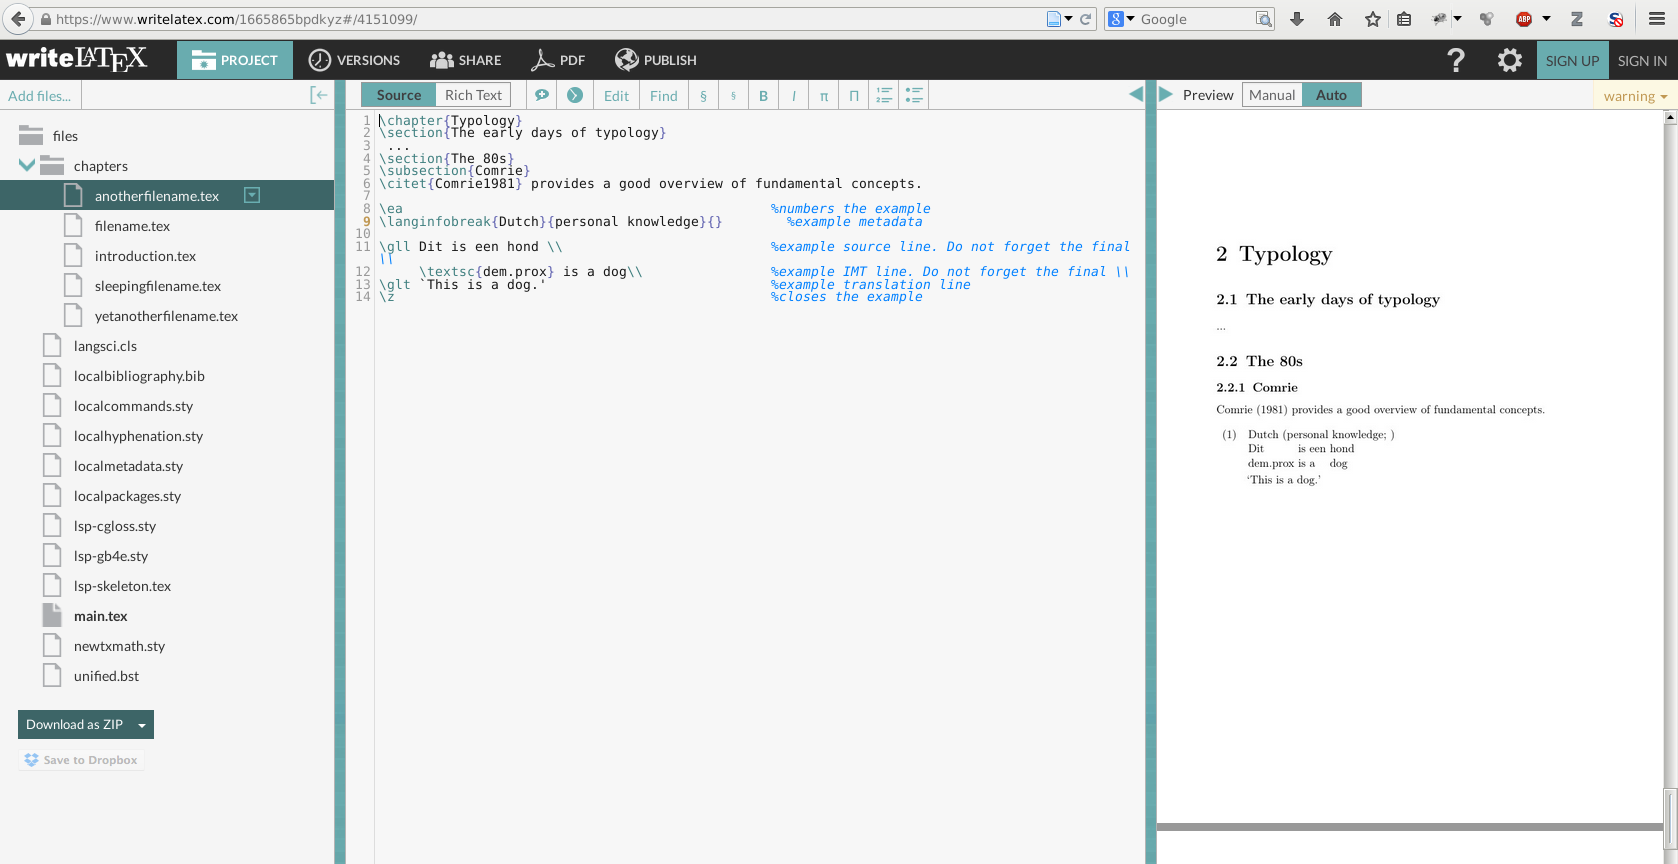
\includegraphics[width=\textwidth]{writelatex.png}
  \caption{Writelatex}
  \label{fig:latex:writelatex}
\end{figure}

\section{The skeleton}
The skeleton has a main file, which is called \verb+lsp-skeleton.tex+. You can leave that name or choose a name more suitable for your book, e.g. \verb+smith.tex+ or \verb+hawaiiangrammar.tex+. That main file draws information from a number of other files which are in the same directory. All those files start with \verb+local...+. Furthermore, the main file includes the chapters, which are found in the directory \verb+chapters/+.

\begin{table}[htb]
  \caption{File structure of the skeleton}
  \label{tab:latex:skeleton}
  \begin{tabular}{lp{6cm}}
    \lsptoprule
    file & content \\
    \midrule
    \verb+localmetadata.sty+ & information about the author, the title, the ISBN etc \\
    \verb+localpackages.sty+ & extra packages you might require, for instance for syntactic trees or Hebrew text\\
    \verb+localcommands.sty+ & extra commands you might want to define, e.g. for very frequent abbrevations in your text\\
    \verb+localhyphenation.sty+ & for words where the \latex hyphenation algorithm does not produce the desired result      \\
    \verb+localbibliography.bib+ & your bibliography in \bibtex-format \\
    \verb+chapters/chapter1.tex+ & text \\
    \verb+chapters/chapter2.tex+ & text \\
... & text \\
    \lspbottomrule
  \end{tabular}
\end{table}

A number of auxiliary files are generated on the fly, these are  \verb+.toc+ for the table of contents; \verb+.bbl+ for the bibliography; and \verb+.ind+, \verb+.and+, and \verb+.lnd+ for the indexes.  

\section{Using the \texttt{langsci} class}
There are a variety of programs for making writing \latex documents easier.

For Microsoft Windows, Texniccenter is the most popular one (\figref{fig:latex:texniccenter}).
For Mac, Texshop (\figref{fig:latex:texshop}) and Texstudio (\figref{fig:latex:texstudio}) are popular choices.
For Linux, Kile is a very good \latex editor (\figref{fig:latex:kile}).

\begin{figure}
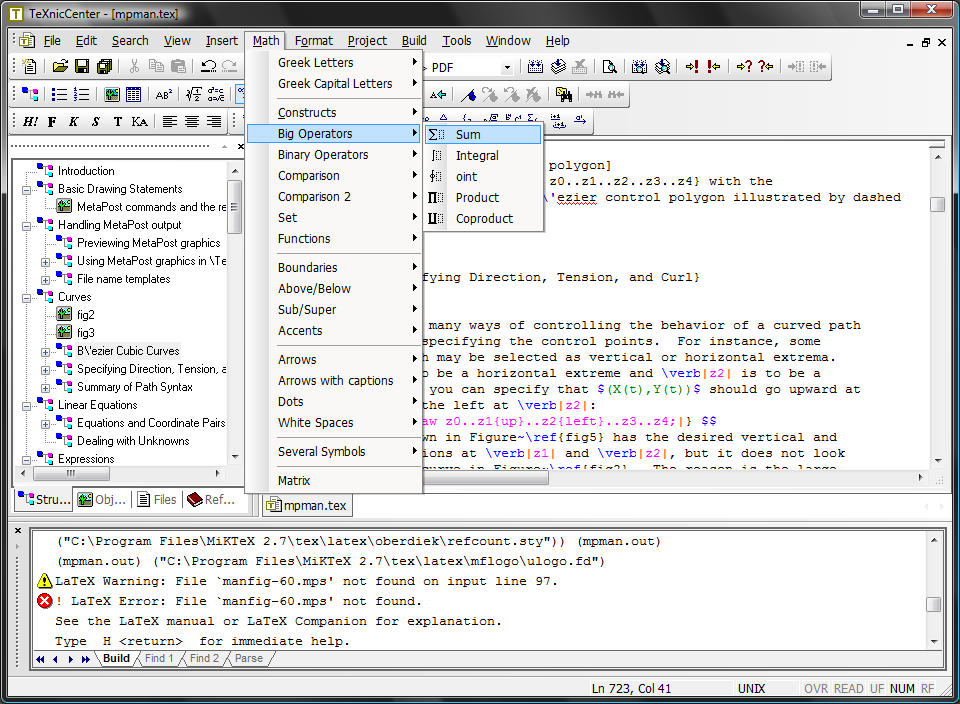
\includegraphics[width=\textwidth]{texniccenter.png}
\caption{Texniccenter}
\label{fig:latex:texniccenter} 
\end{figure}


\begin{figure}
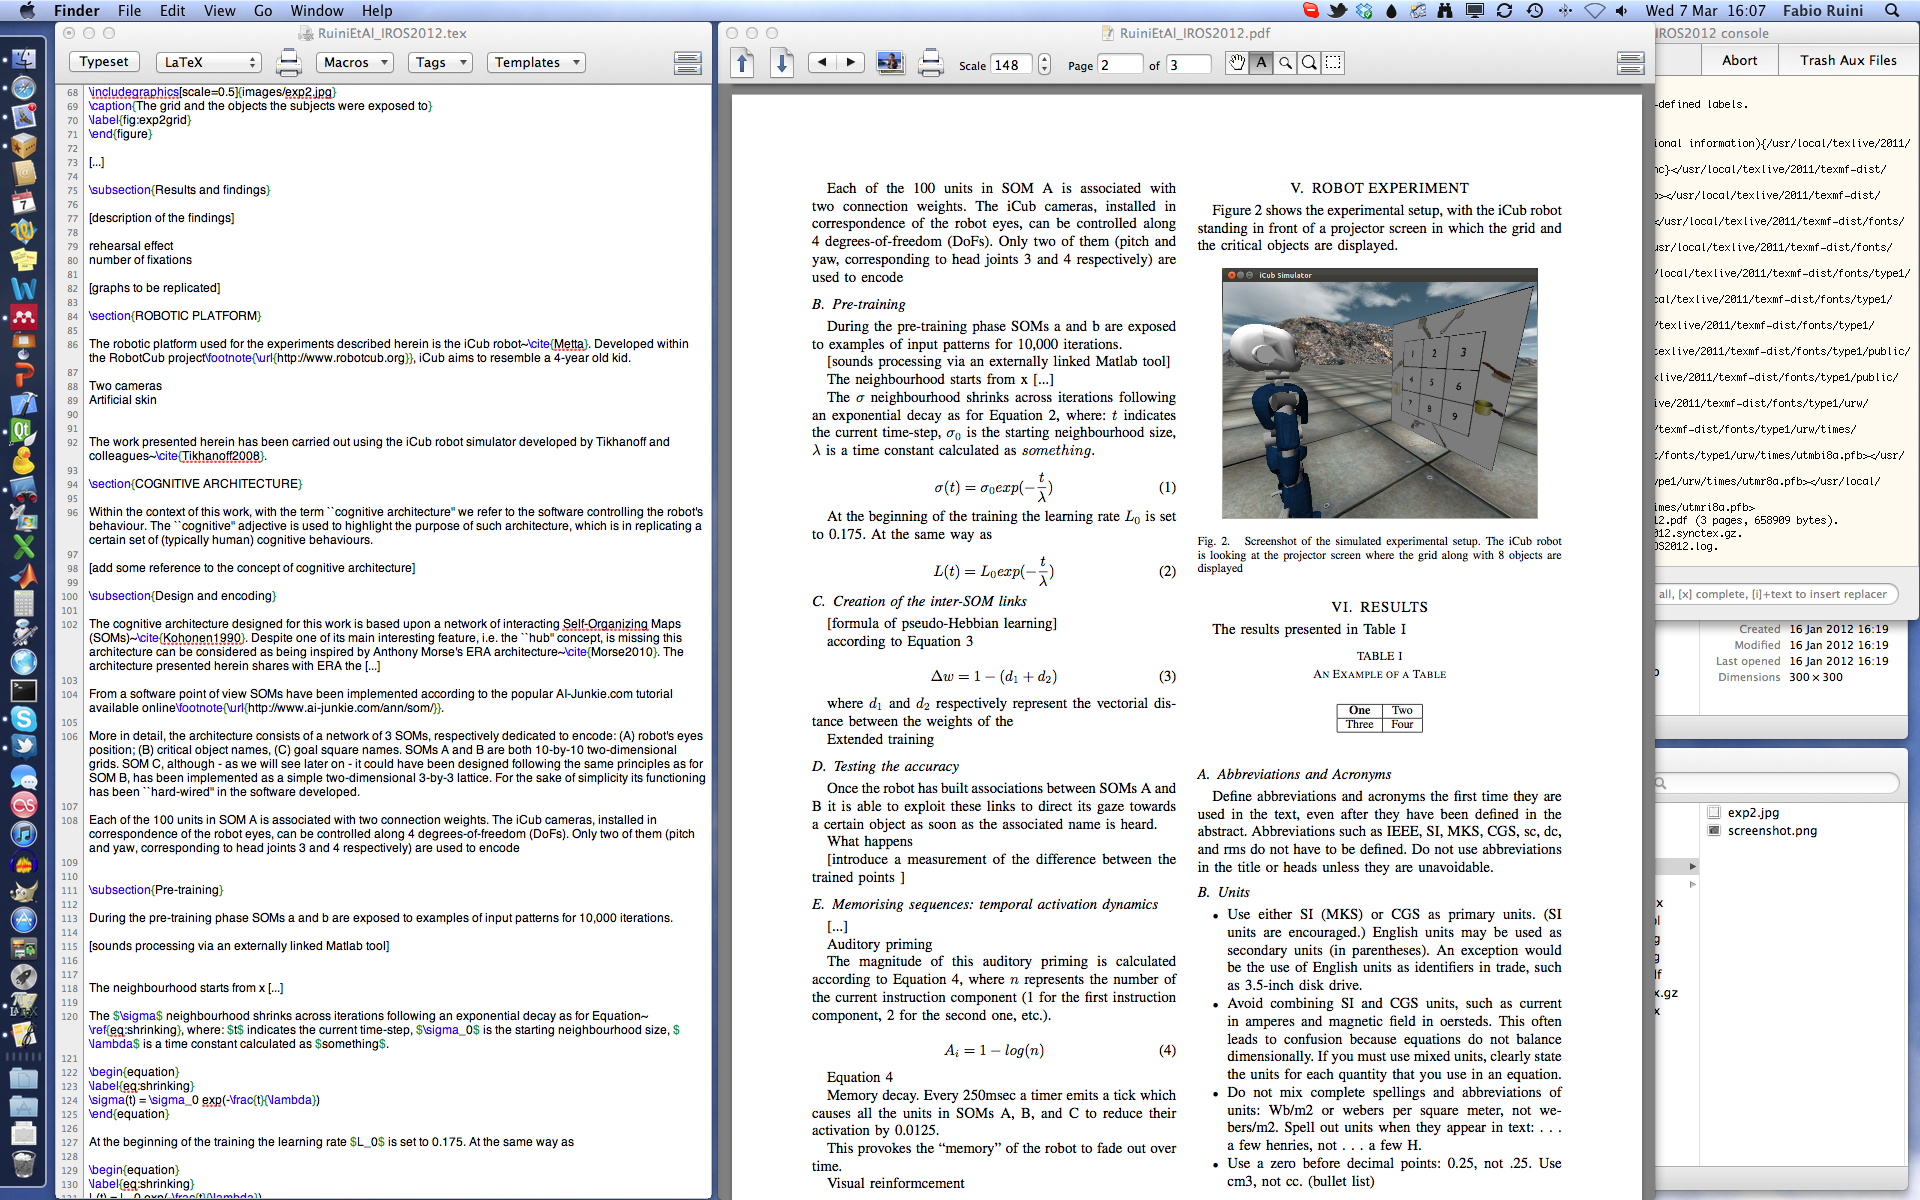
\includegraphics[width=\textwidth]{texshop.png}
\caption{Texshop}
\label{fig:latex:texshop} 
\end{figure}

\begin{figure}
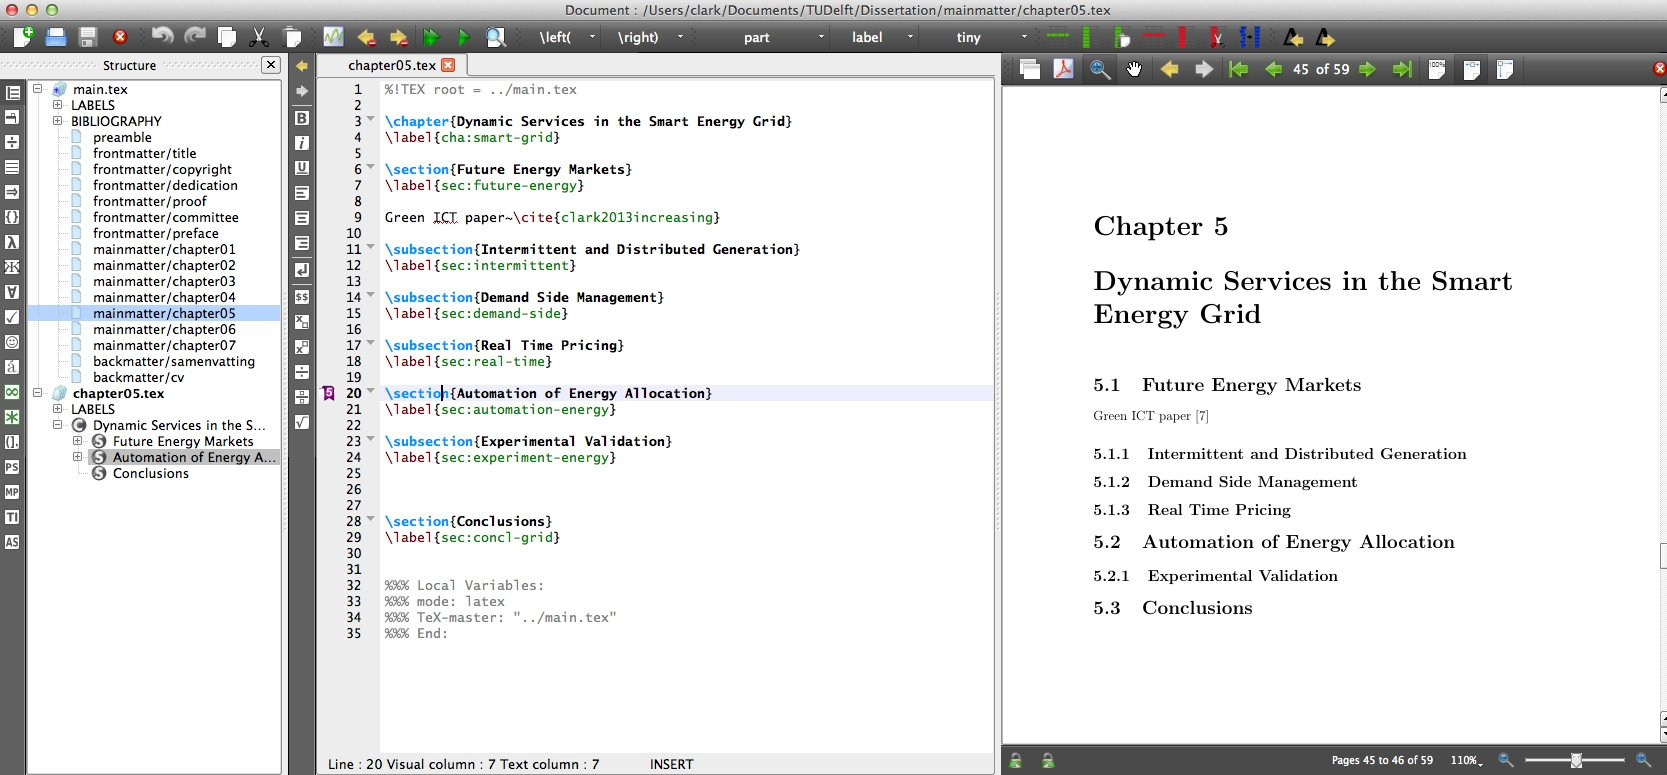
\includegraphics[width=\textwidth]{texstudio.jpg}
\caption{Texstudio}
\label{fig:latex:texstudio} 
\end{figure}


\begin{figure}
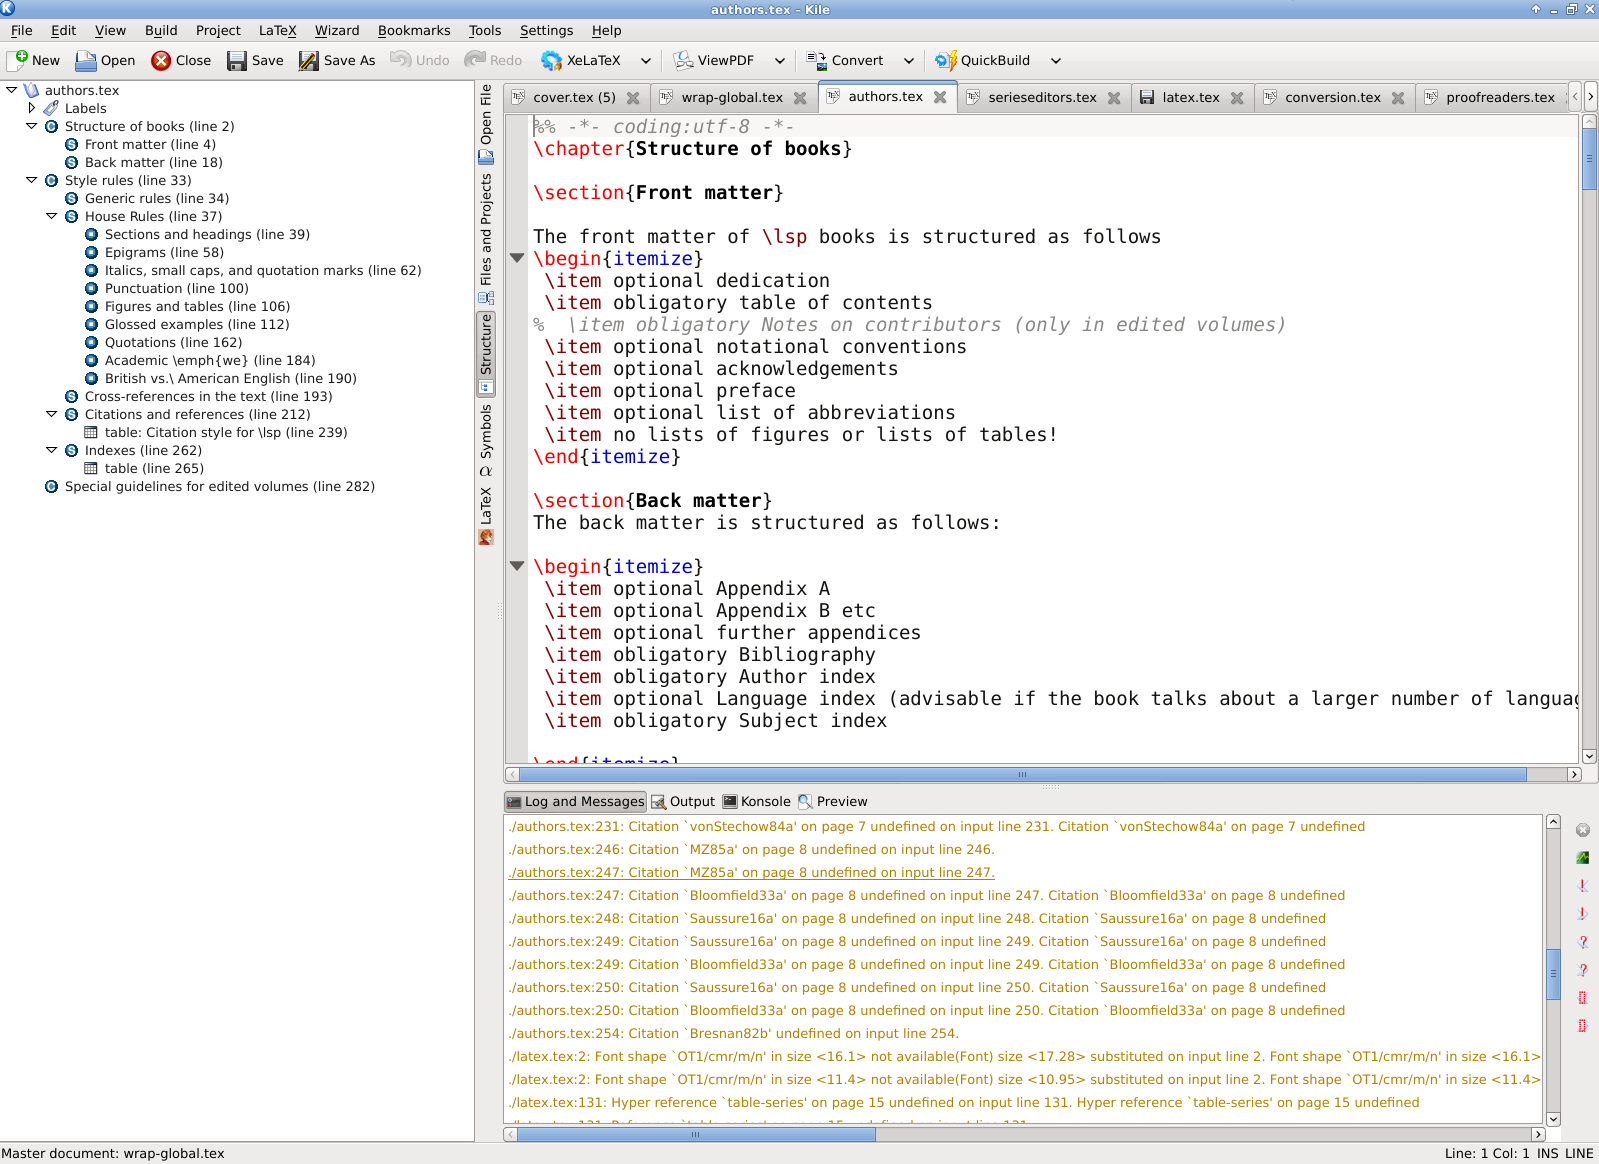
\includegraphics[width=\textwidth]{kile.png}
\caption{Kile}
\label{fig:latex:kile} 
\end{figure}

  
% \subsection{Included packages}
% The following packages are already loaded by default: 
% \verb+amssymb+, 
% \verb+authorindex+, 
% \verb+biblatex+, 
% \verb+booktabs+, 
% \verb+chngcntr+, 
% \verb+chngcntr+, 
% \verb+datetime+, 
% \verb+epigraph+, 
% \verb+etex+, 
% \verb+floatrow+, 
% \verb+fontspec+, 
% \verb+geometry+, 
% \verb+graphicx+, 
% \verb+hyperref +, 
% \verb+ifxetex+, 
% \verb+index+, 
% \verb+microtype+, 
% \verb+natbib+, 
% \verb+newtxmath+, 
% \verb+pbox+, 
% \verb+pst-barcode +, 
% \verb+rotating+, 
% \verb+scrpage2+, 
% \verb+showidx+, 
% \verb+textpos+, 
% \verb+tocstyle+, 
% \verb+url+, 
% \verb+xcolor+, 
% \verb+xspace+, 
% \verb+xstring+. 
% 
\section{Producing the document}
In your \latex editor, there are various ways to create a pdf from your sourcecode. Choose \verb+xelatex+. The first time you run it, it will produce a pdf with all the text, but with no table of contents. When you run it again, you will see the table of contents and the text. There are chances that your editor will show error messages. Common causes are unmatched braces or \verb+\begin{...}+ not followed by \verb+\end{...}+

In order to include the bibliography, you have to run \verb+bibtex+ to read the bibliography, and then again \verb+xelatex+ to include it into your document. Pay attention to error messages and warnings.

\newpage
The creation of the indexes is a bit more complicated. You can leave this to the \lsp people. The relevant commands are:

\begin{verbatim}
makeindex -o lsp-skeleton.ind lsp-skeleton.idx
makeindex -o lsp-skeleton.lnd lsp-skeleton.ldx 
makeindex -o lsp-skeleton.snd lsp-skeleton.sdx
\end{verbatim} 


\section{Adapting the structure of the document}
The general structure of the document is given by \lsp. You have a couple of options to change the structure:
\begin{itemize}
 \item You can choose the skeleton for monograph or edited volume
 \item You can add additional chapters to the directory \verb+chapters+, for instance\\ \verb+chapters/chapter4.tex+ or \verb+chapters/introduction.tex+. Make sure to add \verb+\chapter{Introduction}
This document describes how to create a manuscript with Language Science Press. It discusses what authors, volume editors and the auxiliary roles of proofreaders, typesetters and indexers have to know in order to produce high quality books.
+ (without \verb+.tex+) to your main file.
 \item You can add a preface, acknowledgements, or a list of abbreviations with\\ \verb+\addchap{Preface}+.
 \end{itemize}



\section{Common commands}\label{sec:latex:commoncommands}
The wealth of commands available in \latex can be daunting at first sight. However, very soon you will see that you can get a very long way with some very basic commands. The first batch involve the structure of your document, i.e. the various levels of headings. These are:
\begin{itemize}
 \item \verb+\chapter{titleofheading}+
\item \verb+\section{titleofheading}+
\item \verb+\subsection{titleofheading}+
\item \verb+\subsubsection{titleofheading}+
\end{itemize}

These commands give you a numbered title in the right layout. For prefaces, acknowledgements etc., which are not numbered, use \verb+\addchap{Preface}+ instead of \verb+\chapter{Preface}+. 
Other common commands are 
\verb+\label{la+ \verb+belname}+ 
to assign a label, and 
\verb+\ref{labelname}+
to refer to a label. It is good practice to use 
\verb+\sectref{labelname}+,
\verb+\tabref{labelname}+,
\verb+\figref{labelname}+,
to refer to sections, tables, and figures, respectively. A reference to this section will be \verb+see \sectref{sec:latex:commonco+ \verb+mmands}+, which will produce ``see \sectref{sec:latex:commoncommands}''.

Other commands very often used in academic texts are \verb+\citet{somework}+ and \verb+\citep{somework}+. Use the former to cite a work in the running text and the latter to cite it in parentheses. In order to avoid double parentheses, you can use  \verb+\citealt{somework}+. Page numbers are added with \verb+\citet[99+ \verb+--123]{somework}+. Make sure to use a double hyphen for ranges, which will give a dash in the pdf. Citations work with keys from your \bibtex file. In the examples above \verb+somework+ is the key of a record in your \bibtex file. When \verb+somework+ is cited in the document, the pdf will show the right citation in the right style, and the work will be added automatically to the list of references at the very end. Please refer to the guidlines for bibliographies for more information.


If some text should not be in the normal font, use 
\verb+\textit{text to chan+ \verb+ge}+ for italics, 
\verb+\textsc{text to change}+ for small capitals. There is generally no need to use boldface. If you want to use boldface, get in touch with your series editors.

\subsection{Linguistic examples}
Linguistic examples are typeset like this

\begin{verbatim}
\ea\label{ex:examplelabel}
\langinfo{French}{Indo-European}{personal knowledge}\\
\gll  Jean aim-e                    Marie \\
      John love-\textsc{3s.pres.ind} Mary \\
\glt `John loves Mary.'    
\z
\end{verbatim}

This gives you
% \todo{fix index}
\ea\label{ex:examplelabel}
\langinfo{French}{Indo-European}{personal knowledge}\\
\gll  Jean aim-e Marie \\
      John love-{3\sg.\prs.\ind} Mary \\
\glt `John loves Mary.'    
\z

Rough alignment of glosses in the source text can be helpful, but is not necessary.
Most glosses from the Leipzig Glossing Rules can be accessed via shortcuts. The example above could also be typeset as

\begin{verbatim}
\ea\label{ex:examplelabel}
\langinfo{French}{Indo-European}{personal knowledge}\\
\gll  Jean aim-e                 Marie \\
      John love-{3\sg.\prs.\ind} Mary \\
\glt `John loves Mary.'    
\z
\end{verbatim}

For more complicated examples with more lines, judgments, additional information and the like, refer to the showcases section, or to the documentation of the package \verb+lsp-gb4e+.
\verb+\langinfo+ should be used if the language cannot be assumed to be widely known. The first argument is the language, the second the family, the third the source. If the family is left blank, it will not display. If you give a reference in the source, use \verb+\citealt+ rather than \verb+\citep+.

\subsection{Graphics}
In order to add a graphic, use the following stretch of code

\begin{verbatim}
\begin{figure}
  \includegraphics[height=.3\textheight]{filename.png}
  \caption{Some good caption.}
  \label{fig:chapterhandle:keytofigure}
\end{figure}
\end{verbatim}

\subsection{Tables}
In order to add a table, use the following stretch of code:

\begin{verbatim}
\begin{table} 
  \begin{tabular}{lll}
    \lsptoprule
    German  & French  & Spanish \\
    \midrule
    Zelle   & cellule & célula    \\
    Zelle   & cellule & célula    \\
    Zelle   & cellule & célula    \\
    \lspbottomrule
  \end{tabular}
  \caption{Some good caption.}
  \label{tab:chapterhandle:keytotable}
\end{table}
\end{verbatim}

This will give you  \tabref{tab:chapterhandle:keytotable}. There are ways to add additional vertical lines, but this should generally not be done. If your cells get to wide, use \verb+\begin{tabular}+ \verb+{p{4cm}p{4cm}p{4cm}}+, rather than \verb+\begin{tabular}{lll}+
\begin{table}[h]
  \begin{tabular}{lll}
    \lsptoprule
    German  & French  & Spanish \\
    \midrule
    Zelle   & cellule & célula    \\
    Zelle   & cellule & célula    \\
    Zelle   & cellule & célula    \\
    \lspbottomrule
  \end{tabular}
  \caption{Some good caption.}
  \label{tab:chapterhandle:keytotable}
\end{table}

You should not assume that a figure or table will be placed exactly where it appears in the text. Therefore, references like ``in the table above/below'' should not be used. 

\subsection{Footnotes}
In order to add footnotes, use the command \verb+\footnote{...}+. If you want to use a footnote in an example, use \verb+word {\footnotemark} word word}+ and add a line with \verb+\footnotetext{text of the footnote}+ just before the translation of the example. You should not add footnotes to tables or figures.


A common requirement is to put pages in landscape orientation rather than portrait. In order to do this, use \verb+sidewaysfigure+ or \verb+sidewaystable+ instead of the normal \verb+figure+ or \verb+table+.

Another common requirement is fitting a table or other element which is a bit too large on the page. In order to do this, use \verb+\resizebox{\linewidth}{!}+ \verb+{stuff to resize}+.

For other special needs, please contact our coordinator at \url{support@langsci-press.org}. 

\section{Adapting the class to your needs}

Additional packages can be added via \verb+\usepackage{packagename}+ in the file \verb+localpackages.sty+.
Addtional commands can be added via \verb+{\newco+ \verb+mmand{commandname}{commanddefinition}+ in the file \verb+localcomm+ \verb+ands.sty+. 


Different subdisciplines of linguistics have different requirements. Syntactic trees, generously stacked diacritics, attribute-value matrices, foreign scripts (possibly right-to-left) or OT-tableaus come to mind. Have a look at the `showcases' guideline to see how to typeset these elements.


 
   
\section{Drafts}

Since \lsp does not have any commercial interest, you can put your book on webpages and distribute it
freely. We encourage authors to do this in order to discuss the work and improve it before final
publication. If authors want to circulate prefinal versions, they can use the option
\texttt{draftmode}. This prints a large watermark onto the first page and adds a footer to ever page
that informs the reader about the fact that they are reading a draft and the date and time of the
creation of the draft.
  